\documentclass[aps,prd,superscriptaddress,onecolumn,nofootinbib,preprintnumbers,notitlepage]{revtex4-1}
\usepackage[utf8]{inputenc}
\usepackage{amsmath,amssymb,mathtools}
\usepackage{tabularx}
\usepackage{siunitx}
% \usepackage{authblk}
% \usepackage{standalone}
% \usepackage{xspace}
% \usepackage{hyperref}



\newcommand{\CM}{\mathrm{CM}}
\newcommand{\diff}{\mathrm{d}}

\begin{document}

\title{$S$-matrix approach to the $\rho-\omega$ interference}
\author{Misha~Mikhasenko}\affiliation{CERN-EP, CH-1211, Geneva, Switzerland}\affiliation{JPAC}
\author{others}\affiliation{JPAC}

\nopagebreak
\maketitle

\section{Construction of the scattering matrix}

Here we explore an idea to introduce $\rho-\omega$ interference by a small coupling
between two channels:
\begin{itemize}
  \item $J^{PC}=1^{--}$: $\pi\pi\,P$-wave
  \item $J^{PC}=1^{--}$: $\rho\pi\,P$-wave.
\end{itemize}

The production amplitude $A$ is calculated from the scattering matrix as follows.
\begin{equation}
  A_{\pi\pi} = \hat{A}_{\pi\pi} B_1^{1/2}(p),
\end{equation}
where $p = \sqrt{s/4-m_\pi^2}$ is a pion break-up momentum,
$B_1(p)$ is a threshold factor (+ barrier factor, e.g.\ the Blatt-Weisskopf function, $B_1(p) = p^2/(1+R^2p^2)$, $R=5/$GeV). %,$\alpha_1$, and $\alpha_1$ are the real production coefficients.
% The reduced $T$ matrix is constructed from $K$ matrix in a standard way,
\begin{align} \label{eq:T.2x2}
  T &= \left[1-i K \rho \right]^{-1} T\\
  A &= \left[1-i K \rho \right]^{-1} N.
\end{align}
where $\rho$ is a diagonal matrix, $\rho = \text{diag}(\rho_1,\rho_2)$ with $\rho_1 = \sqrt{1-4m_\pi^2/s}\,\,B_1(p)$, and $\rho_2 = 1$.

The $K$-matrix contains a pole at every channel and a small non-diagonal coupling between two channels.
\begin{equation} \label{eq:K}
  K = \frac{1}{m_1^2-s}\begin{pmatrix}
    g_1^2 & 0\\
    0 & 0
  \end{pmatrix} +
  \frac{1}{m_2^2-s}\begin{pmatrix}
    h^2 & hg_2\\
    hg_2 & g_2^2
  \end{pmatrix}
\end{equation}
The coefficient $h^2$ is proportional $\Gamma_{\omega\to 2\pi}$, i.e. extremely small compare to $g_2^2$.

The denominator of the scattering amplitude is proportional to the $\text{det}(\mathbb{I}-i\rho K)$,
that is a product of the $\rho$ and $\omega$ inverse propagators up to the terms proportional to $g_2^2$.
\begin{align}
  D & = (m_1^2-s)(m_2^2-s)^2\,\,\text{det}(\mathbb{I}-i\rho K) \\\nonumber
    % & = h^{2} g_2^{2} \rho_{1} \rho_{2} (m_{1}^{2} - s) + \big(i \rho_{1}
    % \left(g_{1}^{2} (m_{2}^{2} - s) + h^{2} (m_{1}^{2} - s)\right) \\\nonumber
    % &\qquad - (m_{1}^{2} - s) (m_{2}^{2} - s)\big) \left(i g_2^{2} \rho_{2} - m_{2}^{2} + s\right)\\\nonumber
    &= (m_1^2-s-ig_1^2\rho_1)(m_2^2-s-ig_2^2\rho_2)(m_2^2-s) + O(h^2).
\end{align}
Using the $Q$-vector construction of the production vector,
\begin{equation}
  N = K\,[\alpha_1, \alpha_2]^T,
\end{equation}
we obtain an expression for the amplitude:

\begin{align}
\hat{A}_{\pi\pi} &= \alpha_{1} A^\rho + \alpha_{2} A^{\rho/\omega}
\end{align}
where the amplitudes $A^\rho$ and $A^{\rho/\omega}$ are given by the expressions:
\begin{align}
  A^\rho &= \frac{\left(g_{1}^{2} \left(m_{2}^{2} - s\right) + h^{2} \left(m_{1}^{2} - s\right)\right)
    \left(m_{2}^{2} - s - i g_2^{2} \rho_{2}\right) + i h^{2} g_2^{2} \rho_{2} (m_{1}^{2} - s)}{D}
    \\ \nonumber &
    = \frac{g_1^2}{m_1^2-s-ig_1^2\rho_1} + O(h^2) \\ \nonumber
  A^{\rho/\omega} &= \frac{h g_2 \left(m_{1}^{2} - s\right) \left(m_{2}^{2} - s\right)}{D} =
  \frac{h g_2 (m_1^2-s)}{(m_1^2-s-ig_1^2\rho_1)(m_2^2-s-ig_2^2\rho_2)} + O(h^2).
\end{align}
where we indicated a limit with $h\to 0$.

The pole in the numerator of the $A^{\rho/\omega}$ produces a zero at the value of the bare $\rho$ mass.
Since the bare mass does not have physical meaning and can be shifted arbitrary,
the zero does not need to be enforced there. It is removed with the production coefficients:
\begin{align}
  \alpha_1 &= \text{Pol}_m(s), & \alpha_2 &= \frac{\text{Pol}_n(s)}{m_1^2-s},
\end{align}
with $\text{Pol}_i(s)$ being a real polynomial of the order $i$.
One should be able to obtain a decent fit with $m=1$, $n=0$.
The higher order polynomials should be tried for systematic studies.
%
\section{Values for the couplings}
The parameters of the $K$ matrix in Eq.~\eqref{eq:K} are completely fixed by the widths of the resonances
and branching fractions:
\begin{align*}
  g_1^2 & = m_\rho \Gamma_\rho / \rho_1(m_\rho^2),\\
  g_2^2 & = m_\omega \Gamma_\omega\,\text{Br}(\omega\to3\pi) / \rho_2(m_\omega^2),\\
  h^2 & = m_\omega \Gamma_\omega\,\text{Br}(\omega\to\pi\pi) / \rho_2(m_\omega^2).
\end{align*}

% \section{Fit to the $e^{+}e^{-}$ data}

\section{Further improvements}
One can improve analytic structure of the amplitude by replacing the phase-space factors
by their dispersive representation:
\begin{equation} \label{eq:CM}
i\rho_i \to (\CM_i - \text{Re}\,\CM_i(m_i^2)), \quad
\CM_i = \frac{s}{\pi}\int_{4m_\pi^2}^{\infty} \frac{\diff s'\,\rho_i(s')}{s'(s'-s-i\epsilon)}
\end{equation}

Instread of using a constant for the expression for the $\rho\pi\,P$-wave,
the quasi-two-body phase space can be calculated:
\begin{equation}
\rho_2 \to \frac{1}{s} \int_{4m_\pi^2}^{(\sqrt{s}-m_\pi)^2} \frac{\diff \sigma}{2\pi \sigma}\,\,\frac{\lambda^{1/2}(s,\sigma,m_\pi^2) \lambda^{1/2}(\sigma,m_\pi^2,m_\pi^2)}{(m_\rho^2-\sigma)^2 + (m_\rho \Gamma_\rho)^2} B_1(k) B_1(q),
\end{equation}
with $k = \sqrt{\sigma/4-m_\pi^2}$, $q = \lambda^{1/2}(s,\sigma,m_\pi^2)/(2\sqrt{s})$, and
$\lambda(x,y,z) = x^2+y^2+z^2-2xy-2yz-2zx$.

% \begin{equation}
%   K = \frac{1}{m_1^2-s}\begin{pmatrix}
%     g_{13}^2 & 0\\
%     0 & 0
%   \end{pmatrix} +
%   \frac{1}{m_2^2-s}\begin{pmatrix}
%     g_{14}^2 & g_{14} g_{24}\\
%     g_{14} g_{24} & g_{24}^2
%   \end{pmatrix}
% \end{equation}

\newpage

\appendix

\section{Contribution of the higher resonances}
In this section we address contribution of $\rho(1450)$ and $F$-wave
and argue that for the region of $m_{\pi\pi}$ below $0.8\,$GeV these contributions
are irrelevant. $\pi\pi\,P$-wave is essentially elastic below $1\,$GeV,
therefore the scattering/production amplitudes are proportional
to the sine of the scattering phase $\delta_1$.
These scattering phases are well established, e.g. in analysis of the Madrid group~\cite{GarciaMartin:2011cn}.
Fig.~\ref{fig:scatt.phases} shows the phase of the $F$-wave as well as the phase
of $P$-wave in several models. The $F$-wave reaches just $0.02\,$deg. at $m_{\pi\pi}^{(\text{max})}=0.8\,$GeV. compare to $113.1\,$deg. of $P$-wave.
It gives three order of magnitude suppression of the $F$-wave amplitude if the same production strength is used for both waves.
\begin{figure}
  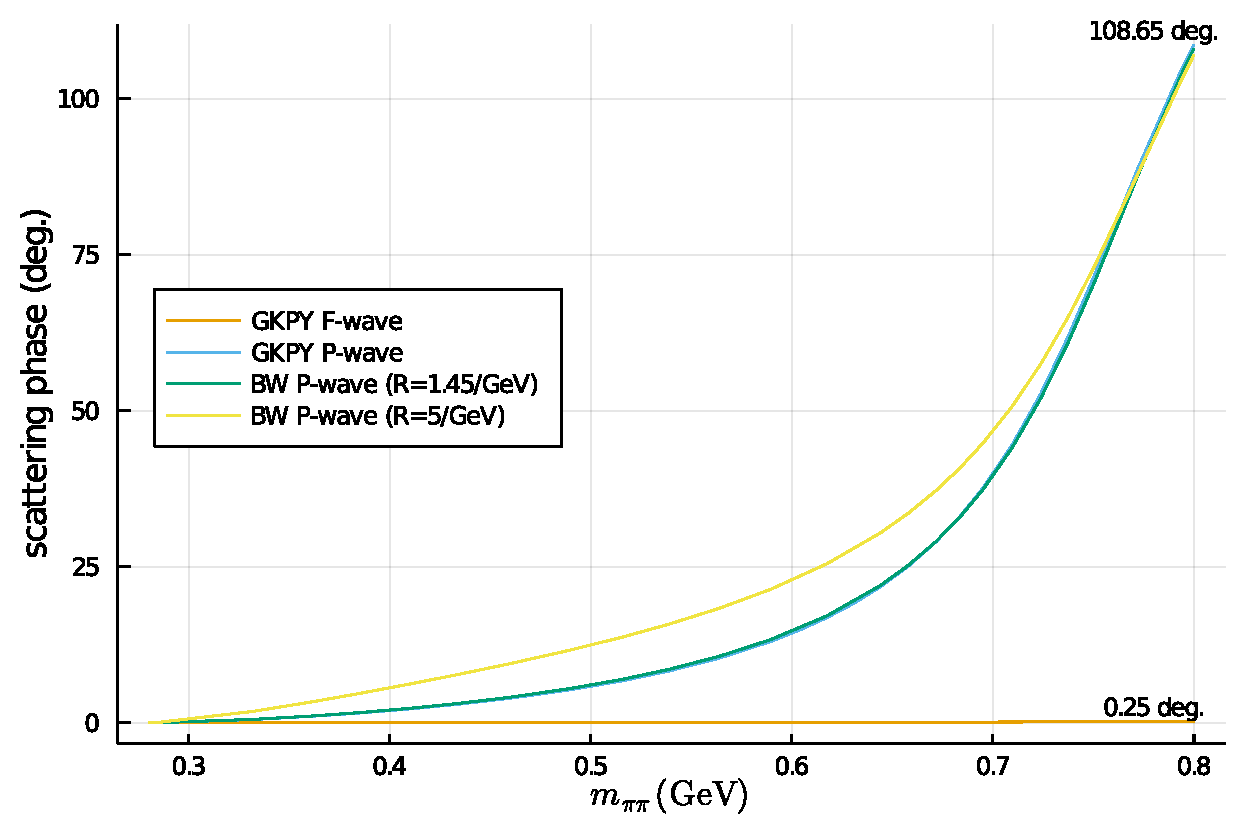
\includegraphics[width=0.7\textwidth]{plots/Pwave_phaseshift.pdf}
  \caption{The $\pi\pi$ P-wave and F-wave scattering phases from the phenomenological analysis of Ref.~\cite{GarciaMartin:2011cn} and the single-pole amplitude with CM function.
  Note that the green line is right on top of the blue line with a little deviation at the limit of the phase space.}
  \label{fig:scatt.phases}
\end{figure}

The phase shift of the $P$-wave for the standard Breit-Wigner amplitude to the one extracted from phenomenological analysis~\cite{GarciaMartin:2011cn} shows a large difference (compare yellow curve and the blue curve)

The difference almost vanishes once the size parameter $R$ is tuned to $0.5/$GeV and the Chew-Mandelstam function, Eq.~\eqref{eq:CM} is used for the energy-dependent width.
The further difference between the Madrid phase (orange line) shows and the adjusted curve
shows potential contributions of the other poles, i.e. $\rho'(1450)$.

\section{Adam's model}
Adam suggested writing amplitude in a form:
\begin{align*}
  T_{11} = \dots\\
  T_{12} = \dots\\
  T_{13} = \dots\\
  T_{14} = \dots\\
\end{align*}
One find the matrix representation of these equations:
\begin{equation} \label{eq:T4x4}
  T = G + G\,\Sigma\,T,
\end{equation}
where
\begin{align}
  G &=
  \begin{pmatrix}0 & 0 & g_{13} & g_{14}\\0 & 0 & 0 & g_{24}\\g_{13} & 0 & 0 & 0\\g_{14} & g_{24} & 0 & 0\end{pmatrix},&
  \Sigma &=
  \begin{pmatrix}
    \rho_1 & 0 & 0 & 0\\
     0 & \rho_2 & 0 & 0\\
     0 & 0 & \frac{1}{m_1^2-s} & 0\\
     0 & 0 & 0 & \frac{1}{m_2^2-s}.
  \end{pmatrix}.
\end{align}
Solving Eq.~\eqref{eq:T4x4} for $T$, we find that it is exactly equivalent to Eq.~\eqref{eq:T.2x2},
with the following correspondence in Eq.~\eqref{eq:K},
\begin{align}
  g_{13} &\Rightarrow g_1,&
  g_{14} &\Rightarrow h,&
  g_{24} &\Rightarrow g_2.
\end{align}

\section{Other check with different production amplitude}
$P$-vector production gives more flexible parametrization
\begin{equation}
  N_i = \sum_R \left( \frac{\alpha_i^R}{m_R^2-s} + f_i \right).
\end{equation}
With an assumption that direct decay of $X$ to $J/\psi\,3\pi$ is negligible, i.e. $f_2 = 0$, we get:
\begin{align}
  \hat{A}_{\pi\pi} &=
    \frac{1}{m_1^2-s-ig_1^2\rho_1} \left(
    \alpha_1^{\rho} + \frac{k \alpha_2^\omega (i\rho_2) (m_1^2-s)}{(m_2^2-s-ig_2^2\rho_2)(m_2^2-s)}
  \right)  + \frac{f_1(m_1^2-s)}{m_1^2-s-ig_1^2\rho_1}\\\nonumber
  &=
    \frac{1}{m_1^2-s-ig_1^2\rho_1} \left(
    \alpha_1^{\rho\prime} + \frac{k \alpha_2^\omega (m_1^2-s)}{m_2^2-s-ig_2^2\rho_2}
  \right)  + \frac{f_1(m_1^2-s)}{m_1^2-s-ig_1^2\rho_1}
\end{align}

\subsection{The final reasonable forms}
We find that unitality-guided amplitude contains two type of terms:
$\rho$-term and $\rho\times\omega$-term with, in principle, arbitrary numerator functions.
The pragmatic approach would be to leave freedom adjust $\rho$-meson lineshape
at the full range of spectrum and allow for local modification in vicinity of the $\omega$ mass.
\begin{align}
  \hat{A}_{\pi\pi}
  & = \frac{c^{\rho} + c^{\pi\pi}(m_1^2-s)}{m_1^2-s-ig_1^2\rho_1}
   + \frac{c^{\rho}}{(m_2^2-s-ig_2^2\rho_2)(m_1^2-s-ig_1^2\rho_1)}\\
  \mathrm{OR,} & =
  \frac{a + bs}{m_1^2-s-ig_1^2\rho_1}\left(
    1+ \frac{c}{m_2^2-s-ig_2^2\rho_2}
  \right).
\end{align}


\bibliographystyle{apsrev4-1}
\bibliography{rho_omega}
\end{document}
